\newpage
\clearpage
\section{Segmentação Panóptica}
\label{panoptic:panoptic}
A segmentação panóptica \cite{Kirillov2019a} é uma nova abordagem que caminha em busca da unificação dos métodos avançados de segmentações, sendo eles: segmentação semântica e segmentação de instâncias \cite{He2020}, as quais foram descritas anteriormente. Baseado nessa abordagem, realiza-se a individualização de objetos e cenas, em que cada pixel das imagens passam a ter um \textit{label} de acordo com a classe do objeto em que o pixel se encontra, assim como um identificador que o diferenciará das demais instâncias mapeadas.

Dentre os objetos que podem ser diferenciados pela segmentação panóptica, duas categorias são nomeadas, portanto, o que as diferenciam, basicamente, é a determinação se o objeto é contável (como pessoa, carro, cachorro e afins), o qual  recebe a denominação de \textit{thing}, ou se o objeto é incontável e/ou amorfo (como céu, terrenos, paredes e semelhantes), o qual seria classificado como \textit{stuff} \cite{Kirillov2019a, Liu2019, Mohan2020}. Vale destacar que objetos pertencentes à classificação de \textit{stuff} não recebem um identificador, pelo fato de ser impossível contá-los ou distinguí-los.

Além disso, no trabalho desenvolvido por \cite{Kirillov2019a}, ficou claro que a rede teve dificuldades para realizar a segmentação de objetos pequenos, todavia, estes resultados não são discrepantes na maioria das vezes, quando comparada às segmentações realizadas por humanos, embora os resultados humanos sejam superiores quando quantificados por métricas de \textit{Panoptic Quality} (PQ), \textit{Segmentation Quality} (SQ) e \textit{Recognition Quality} (RQ), em conjuntos de dados Cityscapes \cite{Cordts2016}, ADE20k \cite{Zhou2016} e Mapillary Vistas \cite{Neuhold2017_ICCV}, que serão discorridas na Seção \ref{panoptic:dataset}, como é possível observar na Tabela \ref{panoptic:table:1} \cite{Kirillov2019a}.

\begin{table}[H]
    \centering
    \caption{Desempenho homem vs máquina.}
    \label{panoptic:table:1}
    \begin{tabular}{@{}l|lll@{}}
    \textbf{Cityscape} & PQ   & SQ   & RQ   \\ \hline
    human              & $69,6^{\substack{+2,5\\-2,7}}$ & $84,1^{\substack{+0,8\\-0,8}}$ &  $82,0^{\substack{+2,7\\-2,9}}$ \\
    machine            & 61,2 & 80,9 & 74,4 \vspace*{0,3cm}\\
    \textbf{ADE20k}    & PQ   & SQ   & RQ   \\ \hline
    human              & $67,6^{\substack{+2,0\\-2,0}}$ & $85,7^{\substack{+0,6\\-0,6}}$ & $78,6^{\substack{+2,1\\-2,1}}$ \\
    machine            & 35,6 & 74,4 & 43,2 \vspace*{0,3cm}\\
    \textbf{Vistas}    & PQ   & SQ   & RQ   \\ \hline
    human              & $57,7^{\substack{+1,9\\-2,0}}$ & $79,7^{\substack{+0,8\\-0,7}}$ & $71,6^{\substack{+2,2\\-2,3}}$ \\
    machine            & 38,3 & 73,6 & 47,7
    \end{tabular}

    \vspace*{1 cm}
    Fonte: retirado e adaptado de \cite{Kirillov2019a}.
\end{table}

Na Figura \ref{panoptic:fig:1} é possível observar as diferenciações realizadas entre as segmentações de instâncias (Figura \ref{panoptic:fig:1}\subref{panoptic:fig:1.1}), contando apenas com o encontro de objetos, a segmentação semântica (Figura \ref{panoptic:fig:1}\subref{panoptic:fig:1.2}), compreendendo classes para cada pixel, mas não diferenciando instancias e, por fim, a segmentação panóptica (Figura \ref{panoptic:fig:1}\subref{panoptic:fig:1.3}) abrangendo \textit{things} e \textit{stuffs}, separando cada uma das instâncias, assim como determinando uma classe para cada pixel.

\begin{figure}[H]
   \caption{Segmentações modernas.}
   \centering
   \label{panoptic:fig:1}
    \begin{subfigure}[t]{0.45\textwidth}
        \centering
        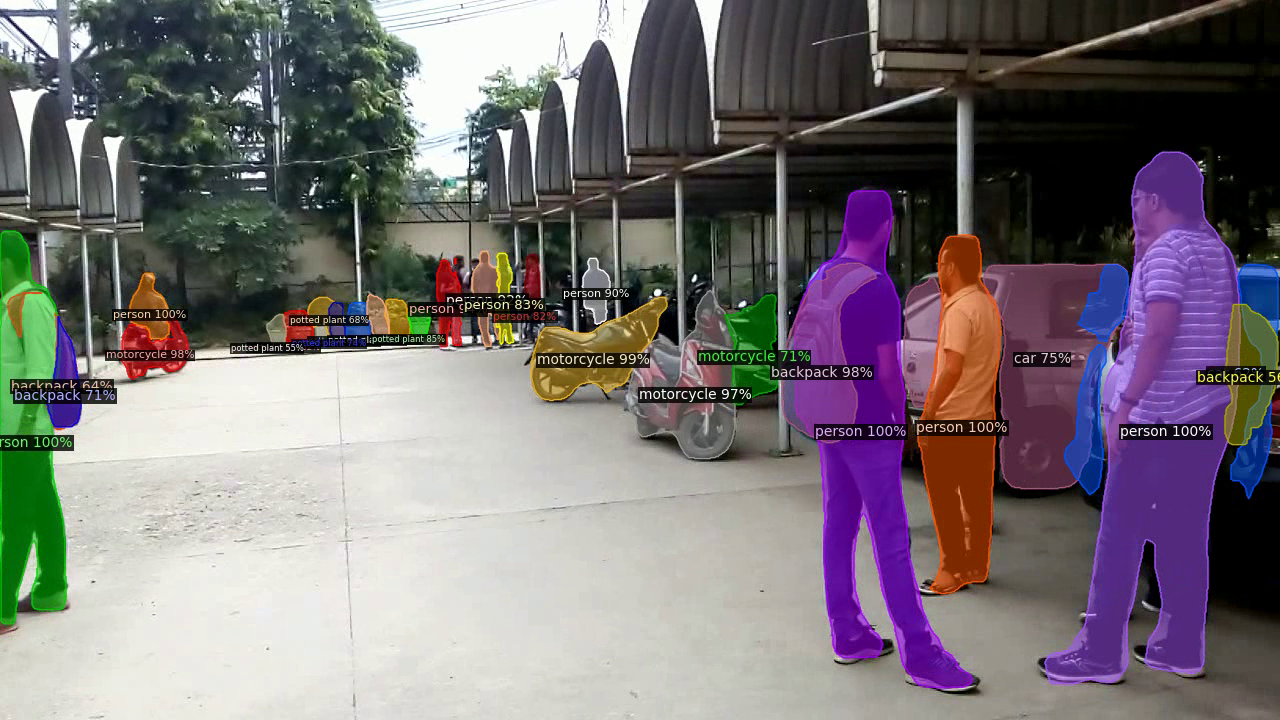
\includegraphics[height=1.5in]{recursos/imagens/panoptic/college_instance.png}
        \caption{Segmentação de instancia.}
        \label{panoptic:fig:1.1}
    \end{subfigure}%
    ~ 
    \begin{subfigure}[t]{0.45\textwidth}
        \centering
        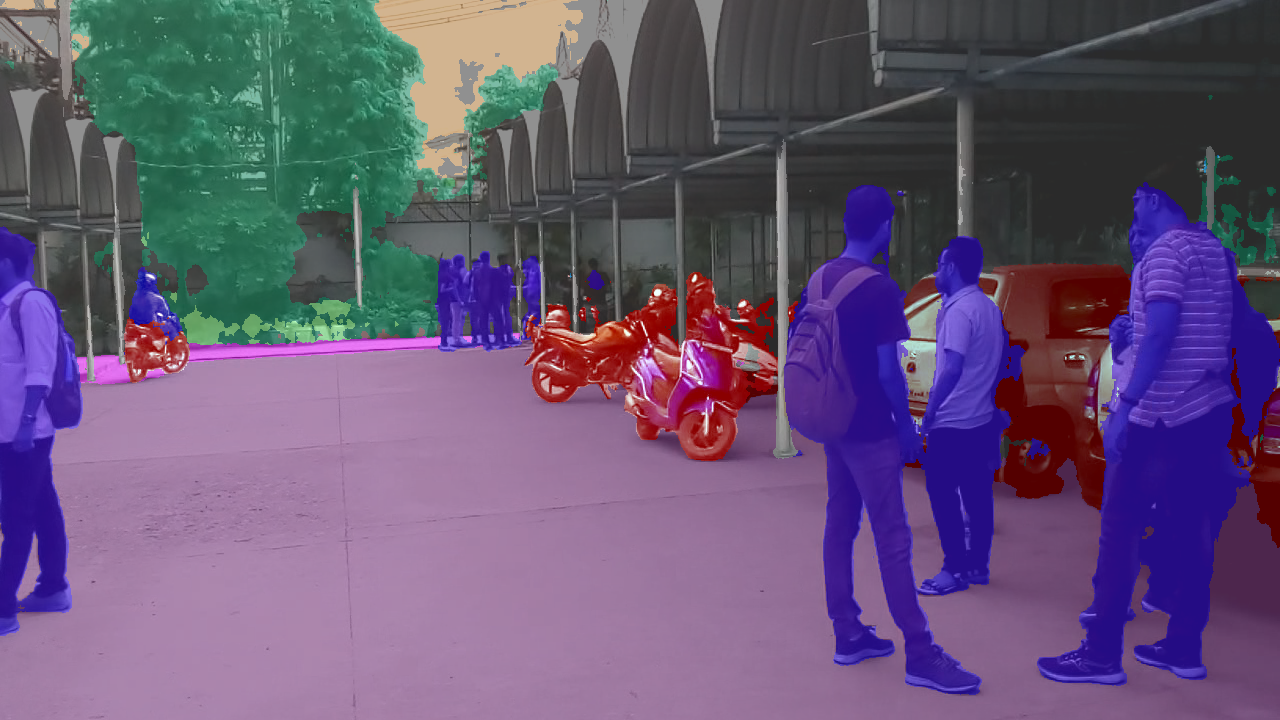
\includegraphics[height=1.5in]{recursos/imagens/panoptic/college_semantic.png}
        \caption{Segmentação semântica.}
        \label{panoptic:fig:1.2}
    \end{subfigure}%
    ~ 
    
    \begin{subfigure}[t]{0.7\textwidth}
        \centering
        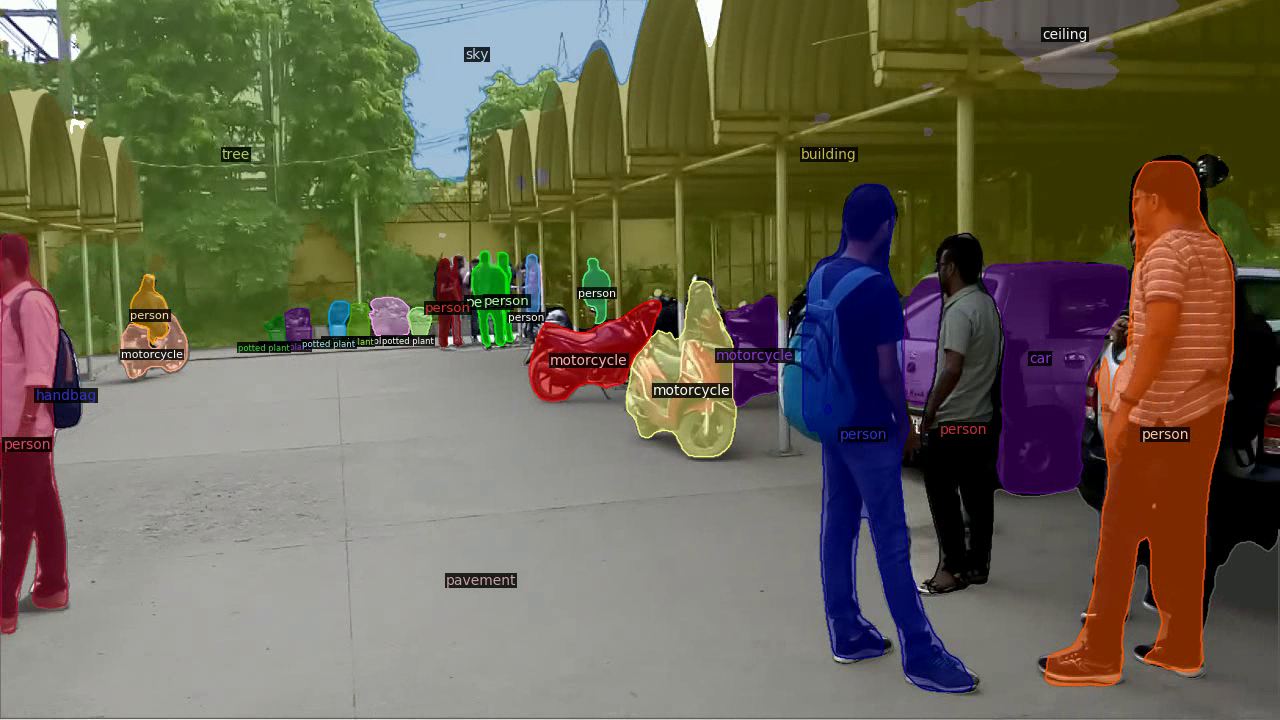
\includegraphics[width=1\linewidth]{recursos/imagens/panoptic/college_panoptic.png}
        \caption{Segmentação panóptica.}
        \label{panoptic:fig:1.3}
    \end{subfigure}

    \vspace*{1 cm}
    Fonte: retirado e adaptado de \cite{Kumar2019IntroductionTutorial}.
\end{figure}

Destarte, a segmentação panóptica caminha contribuindo para os avanços tecnológicos em relação ao entendimento de cenários, carros autônomos \cite{Liu2019} e outras situações em que todos os objetos possuem uma determinada relevância no contexto, como realizado em \cite{Brunger2020} que trabalha com a segmentação panóptica de porcos em chiqueiros.

Nas próximas seções, serão discutidos assuntos relacionados aos conjuntos de dados (Seção \ref{panoptic:dataset}), às arquiteturas (Seção \ref{panoptic:arch}) e às métricas (Seção \ref{panoptic:metrics}) utilizada para a realização de segmentação panóptica, principalmente, no trabalho desenvolvido por \cite{Kirillov2019a}.


\subsection{Conjuntos de dados}
\label{panoptic:dataset}
Mesmo com a amplitude de \textit{datasets} disponíveis para segmentação de imagens, no âmbito da segmentação panóptica se faz necessário um cuidado para a escolha dos mesmos, visto que dentre os requisitos necessários, encontra-se a necessidade de anotação dos pixels e uma identificação das diferentes instâncias, de modo que seja possível diferenciar \textit{things} e \textit{stuffs}.

Dentre os conjuntos de dados trabalhadas inicialmente por Kirillov \textit{et al.} \cite{Kirillov2019a}, vale destacar que três possuíam os requisitos necessários, sendo Cityscapes \cite{Cordts2016}, ADE20k \cite{Zhou2016} e Mapillary Vistas \cite{Neuhold2017_ICCV}, mas destacando também a possibilidade de realizar um trabalho com COCO \cite{Lin2014}, que havia sido anotada recentemente \cite{Kirillov2019a}.

Após este trabalho, outros conjuntos de dados relacionados à segmentação panóptica foram desenvolvidos, dos quais é possível citar o trabalho de Mohan e Valada \cite{Mohan2020}, que acrescentaram os conjuntos de dados KITTI \cite{Geiger2013} e Indian Driving Dataset (IDD) \cite{Varma2018} ao seu trabalho.

Outra opção de conjunto de dados consiste em uma implementação e uso de um conjunto de dados interna, como realizado no trabalho de Xiong \textit{et al.} \cite{Xiong2019}, que fez algo similar ao conjunto de dados Cityscapes e obteve comportamentos parecidos a este e ao conjunto de dados COCO.

De modo geral, a maior parte dos trabalhos realizados consistem em trabalhos com imagens de cidades, carros, metrópoles e afins, como é possível observar na Figura \ref{panoptic:fig:3}. Os conjuntos de dados mais populares, logo, aqueles em que se há uma preferência na escolha são COCO \cite{Caesar2016, Lin2014} e Cityscape \cite{Cordts2016}, como ocorre nos trabalhos \cite{Chen2019, DeGeus2019a, DeGeus2019, Hou2019, Liu2019, Xiong2019}. Vale frisar que as exceções quanto aos conteúdos dos conjuntos de dados também são encontradas em trabalhos de conjuntos de dados de específicos ou privados, como ocorre no trabalhos desenvolvido por Brünger \textit{et al.} \cite{Brunger2020}.

\begin{figure}[H]
   \caption{Imagens de conjuntos de dados de segmentação panóptica.}
   \centering
   \label{panoptic:fig:3}
    \begin{subfigure}[t]{0.40\textwidth}
        \centering
        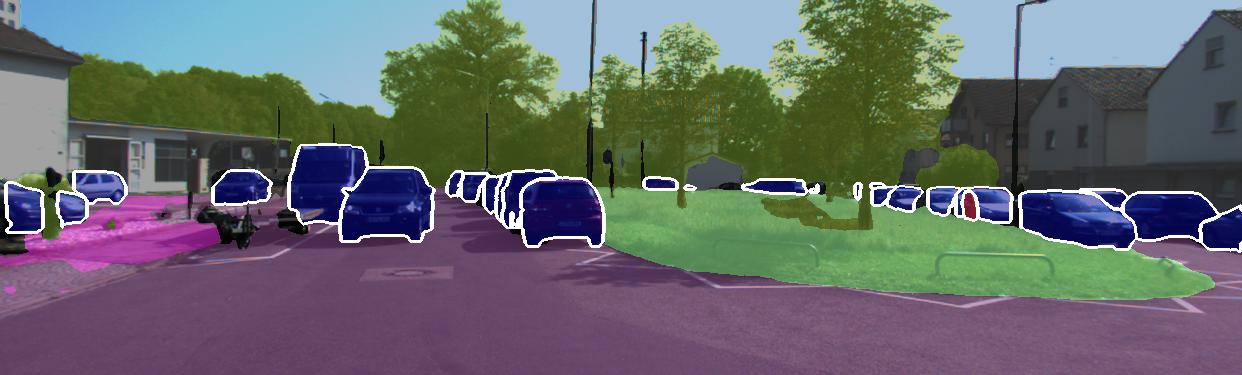
\includegraphics[width=1\linewidth]{recursos/imagens/panoptic/kitti.jpg}
        \caption{Imagem do KITTI \cite{Geiger2013}.}
        \label{panoptic:fig:3.1}
    \end{subfigure}%
    ~ 
    \begin{subfigure}[t]{0.50\textwidth}
        \centering
        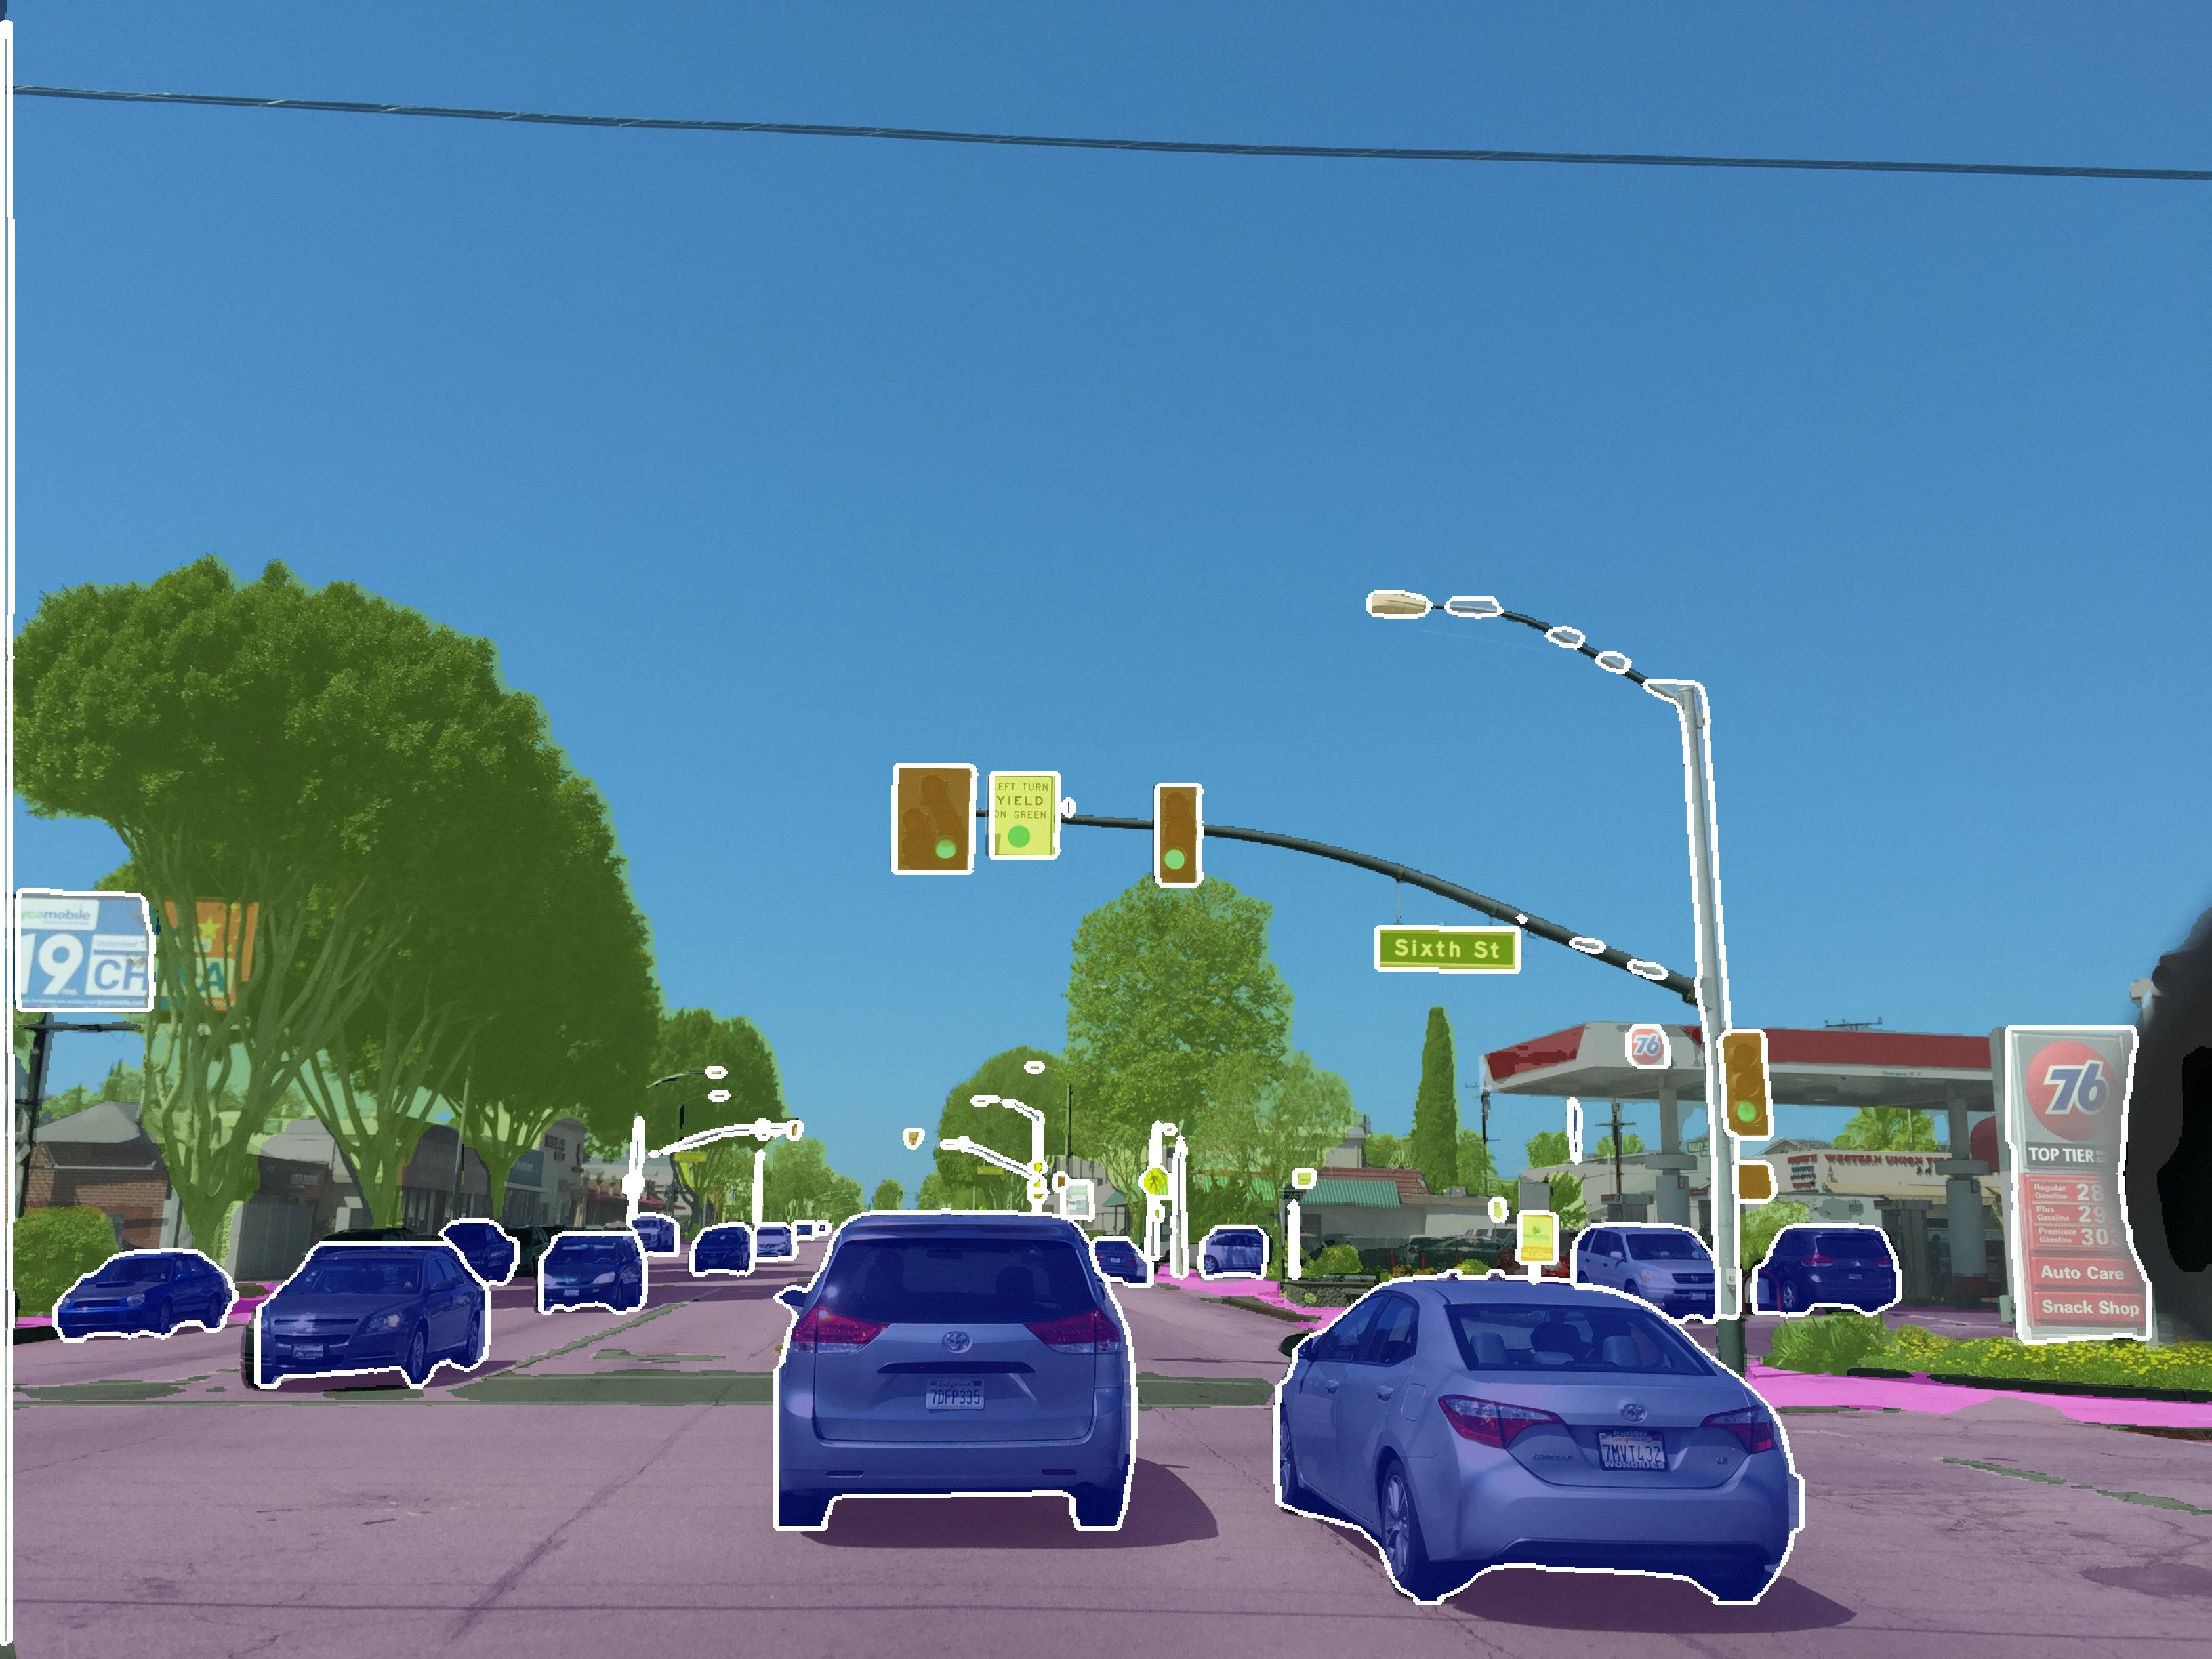
\includegraphics[height=1.3in]{recursos/imagens/panoptic/vistas.jpg}
        \caption{Imagem do Mapillary Vistas \cite{Neuhold2017_ICCV}.}
        \label{panoptic:fig:3.2}
    \end{subfigure}%
    ~ 
    
    \begin{subfigure}[t]{0.45\textwidth}
        \centering
        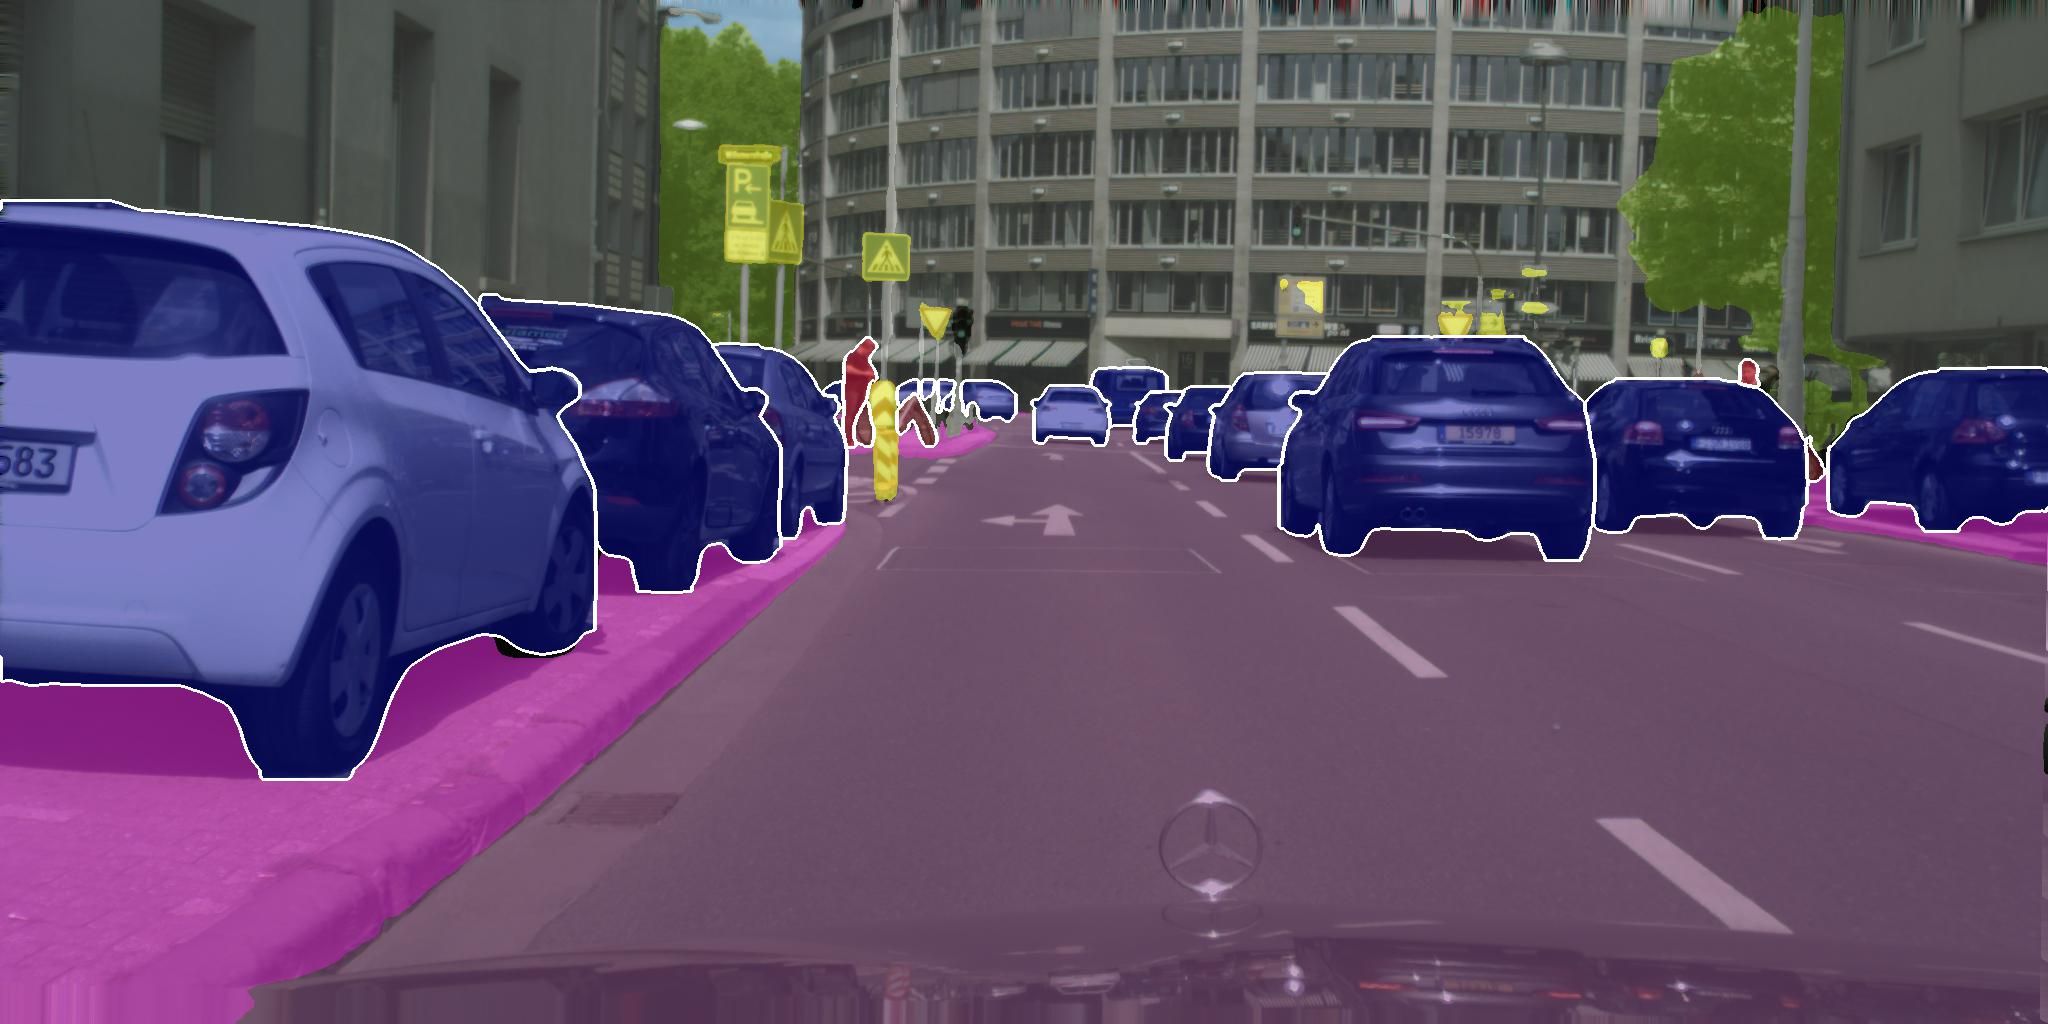
\includegraphics[height=1.3in]{recursos/imagens/panoptic/cityscapes.jpg}
        \caption{Imagem do Cityscapes \cite{Cordts2016}.}
        \label{panoptic:fig:3.3}
    \end{subfigure}
    ~
    \begin{subfigure}[t]{0.45\textwidth}
        \centering
        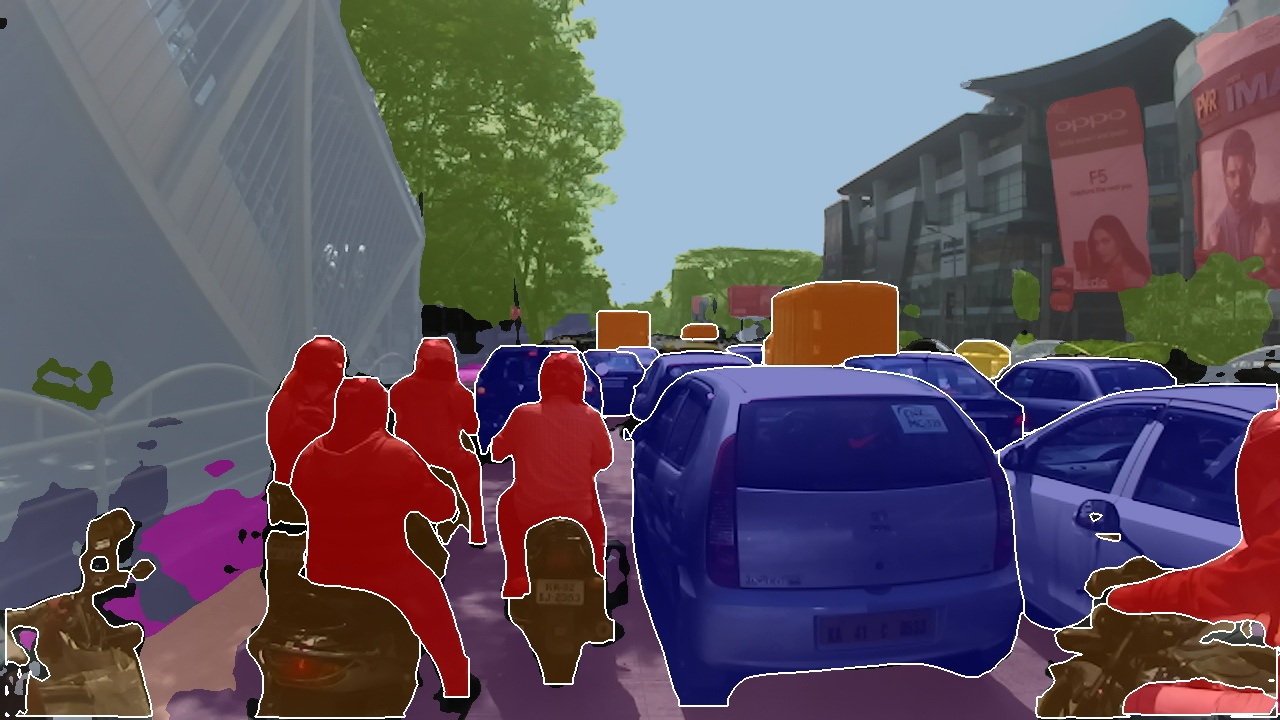
\includegraphics[height=1.3in]{recursos/imagens/panoptic/idd.jpg}
        \caption{Imagem do IDD \cite{Varma2018}.}
        \label{panoptic:fig:3.4}
    \end{subfigure}

    \vspace*{1 cm}
    Fonte: retirado e adaptado de \cite{Mohan2020}.
\end{figure}


\subsection{Arquitetura}
\label{panoptic:arch}
A arquitetura para a formação do modelo de segmentação panóptica, surgiu em um primeiro momento como proposta desenvolvida por Kirillov \textit{et al.} \cite{Kirillov2019a}, comportando duas redes. A primeira das redes tinha o objetivo de realizar a segmentação de instâncias e essa rede era a \textit{Mask} R-CNN \cite{He2020}. A segunda rede, por sua vez, seria responsável pela realização da segmentação semântica, em que dentre as testadas o destaque foi para a rede PSPNet multi-scale \cite{Zhao2017}. A proposta do uso dessas redes dava forma para uma arquitetura robusta e poderosa \cite{Kirillov2019a} por trabalhar com redes consideradas estado da arte para a época.

Todavia, após o término da primeira rede para a realização de segmentação panóptica, outros trabalhos foram realizados, de modo que estes sugeriam novas configurações e levantamentos de pontos diferentes para cada individualidade das configurações adotadas.

Em relação ao desenvolvedor da rede prógona, após os avanços de seus estudos, Kirillov \textit{et al.} \cite{Kirillov2019} desenvolveu uma arquitetura que propunha a unificação de redes, sendo composta por uma rede \hyperref[instance:mask]{Mask R-CNN} com uma \hyperref[semantic:FCN]{FCN}, de sorte que esta unificação proporcionasse efetividade para a segmentação de instâncias e leveza para a segmentação semântica, mas sem perdas em relação ao seu potencial da rede desenvolvida em seu trabalho anterior, segundo \cite{Kirillov2019}. Para realizar a junção dessas redes foi utilizado dos conceitos e estruturas de uma \textit{Feature Pyramid Network} (FPN) \cite{Lin2016}, um extrator de atributos comum para quem deseja acurácia e desempenhos relevantes não só em relação a grandes objetos, mas também aos pequenos \cite{Lin2016} e, assim, suprindo uma das desvantagens pendentes na primeira configuração de arquitetura das redes para segmentação panóptica \cite{Kirillov2019, Kirillov2019a}. Destaca-se, ainda, que esta arquitetura com rede FPN trabalha com uma configuração \textit{top-down} com conexões laterais, de modo que torna possível realizar uma restauração das resoluções com valorosas informações semânticas. As representações de extração de características com estratégia \textit{bottom-up} e a adotada pela FPN - com conexões laterais - podem ser observadas na Figura \ref{panoptic:fig:2}, respectivamente.

\begin{figure}[H]
   \caption{Extrações de características e FPN.}
   \centering
   \label{panoptic:fig:2}
    \begin{subfigure}[t]{0.45\textwidth}
        \centering
        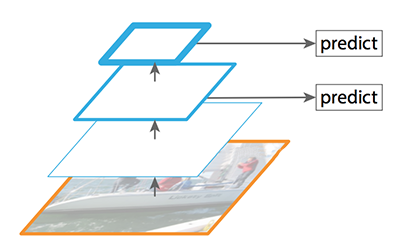
\includegraphics[height=1in]{recursos/imagens/panoptic/bottom-up.png}
        \caption{Configuração \textit{bottom-up}.}
        \label{panoptic:fig:2.1}
    \end{subfigure}%
    ~ 
    \begin{subfigure}[t]{0.45\textwidth}
        \centering
        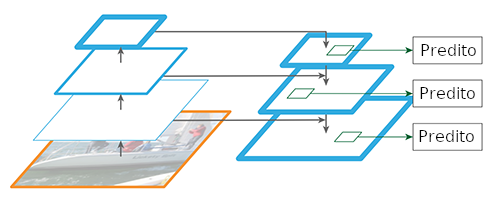
\includegraphics[height=1in]{recursos/imagens/panoptic/FPN.png}
        \caption{FPN.}
        \label{panoptic:fig:2.2}
    \end{subfigure}%

    \vspace*{1 cm}
    Fonte: retirado e adaptado de \cite{Lin2016}.
\end{figure}


\subsection{Métricas}
\label{panoptic:metrics}
Em relação às métricas disponíveis para a avaliação de segmentações panópticas, vale ressaltar que em trabalhos anteriores aos desenvolvidos por Kirillov \textit{et al.} \cite{Kirillov2019a}, a realização da avaliação de \textit{things} e \textit{stuffs} era feita de modo distinto e independente como em \cite{Sun2014, Yao2012}. Com uma proposta que disponibilizasse o trato igualitário para os dois tipos de classificação, significado claro, além de fácil entendimento e implementação , Kirillov \textit{et al.} \cite{Kirillov2019a} elaborou o método de \textit{Panoptic Quality} (PQ) que mensurava a qualidade da segmentação realizada em relação ao \textit{ground truth}, que se efetivava  a partir da realização de dois requisitos: 1) encontro de segmentação e  2) cálculo de PQ.

A primeira das necessidades é cumprida apenas em segmentações que contam com técnicas de \textit{non-overlapping} (sem sobreposição) para que seja possível encontrar uma única segmentação, como \cite{Neubeck2006}, e possuem um valor de IoU superior ou igual à 50\% da área em relação ao \textit{ground truth}, sendo esse valor adequado como parâmetro de limiar, sem que ofereça falsas segmentações e consiga trabalhar tanto com objetos grandes quanto com objetos pequenos, segundo \cite{Kirillov2019a}.

Depois, a segunda das necessidades para a determinação de PQ conta com fórmulas que sugerem a unificação de métricas de SQ e RQ. Além disso, para a determinação dessa formula, se faz necessário o uso de parâmetros que determinarão segmentações condizentes com o \textit{ground truth}, segmentações não encontradas em relação aos preditos e segmentações não encontradas em relação ao \textit{ground truth}, respectivamente, sendo representados por verdadeiro positivo (VP), falsos positivos (FP) e falsos negativos (FN). Logo, a fórmula para determinação de PQ \cite{Kirillov2019a}, em que $p$ representa os preditos e $g$ representa o \textit{ground truth}, pode ser expressa por:

\begin{equation}
\label{panoptic:eq:1}
    PQ = \frac{\sum _{(p,g) \in VP} IoU(p,g)}{|VP|+ \frac{1}{2}|FP| + \frac{1}{2}|FN|}.
\end{equation}

O que remete, também, a uma multiplicação de métrica de qualidade para segmentação por métrica de qualidade para reconhecimento, quando dividida pela quantidade de classificações demarcadas como VP, podendo ser representada por uma segunda fórmula (\ref{panoptic:eq:2}), como sugere Kirillov \textit{et al.} \cite{Kirillov2019a}, e descrita na Equação 30:

\begin{equation}
\label{panoptic:eq:2}
   PQ = \underbrace{\frac{\sum _{(p,g) \in VP} IoU(p,g)}{|VP|}}_{SQ} \times \underbrace{\frac{|VP|}{|VP|+ \frac{1}{2}|FP| + \frac{1}{2}|FN|}}_{RQ}.
\end{equation}

Assim, com a unificação desses parâmetros e formação da PQ, vantagens podem ser observadas quando comparada a métricas de AP (Seção \ref{instance:AP}), por exemplo, que não podem ser utilizadas para segmentações semânticas, ou quando comparadas a métricas de IoU (Seção \ref{semantic:IoU}), que não pode avaliar corretamente classes do tipo \textit{thing}.

Por fim, vale realçar que uma segunda métrica foi desenvolvida para quantificar segmentações panópticas, sendo esta desenvolvida e disponibilizada de modo \textit{open-source} por \cite{Yang2019}, que a nomeou de \textit{Parsing Covering}(PC) e teve iniciativa a partir do trabalho realizado por \cite{Arbelaez2011}. A PC, no que lhe concerne, é uma métrica que não ignora a dificuldade comumente encontrada em redes de segmentação panóptica e concede valor aos tamanhos dos objetos de uma cena, visto que a dificuldade supracitada está na detecção de objetos pequenos. Dessa forma, à fórmula dessa métrica pode ser definida como:

\begin{equation}
    \label{panoptic:eq:3}
    PC = \frac{1}{C} \underset{i=1}{\overset{C}{\sum}}Cov_i,
\end{equation}
sendo,
\begin{equation}
    \label{panoptic:eq:4}
    Cov_i = \frac{1}{N_i}\underset{p \in S_i}{\sum} |p|\cdot \underset{g \in S'_i}{max IoU(p,g)}
\end{equation}
e
\begin{equation}
    \label{panoptic:eq:5}
    N_i = \underset{p \in S_i}{\sum} |p|.
\end{equation}
Nestas Equações \ref{panoptic:eq:3} a \ref{panoptic:eq:4}, $C$ está relacionada à quantidade de classes semânticas, $S'_i$ e $S_i$ são os valores de segmentação predita e de \textit{ground truth}, respectivamente, $N_i$ representa a quantidade de pixels de \textit{ground truth} dentro de $S'_i$, $Con_i$ é a classe coberta pela interação e, finalmente, $PC$ é o valor da métrica estabelecido pela média de $Cov_i$ sobre $C$ classes semânticas, segundo as definições de \cite{Yang2019}.


\subsection{Considerações Finais do Capítulo}
\label{panoptic:conclusion}
Neste capítulo foi possível observar que as segmentações panópticas, embora sejam um assunto relativamente novo, visto que o primeiro trabalho consolidado e que nomeou a rede foi realizado por Kirillov \textit{et al.} \cite{Kirillov2019a} em 2019, esse tipo de segmentação oferece diversos desafios que podem evoluir para as contribuições da ciência, dos quais se destacam:
 
 \begin{itemize}
     \item Segmentação desalinhada, em que a segmentação não cobre a forma correta em relação ao \textit{ground truth};
     \item Perda de contexto, em que há uma confusão entre os ambientes em que as segmentações são realizadas;
     \item Mau alinhamento, em que há falhas em meio a detecção realizada, deformando os formatos dos objetos e cenas.
 \end{itemize}

Esses pontos podem ser observados a partir da Figura \ref{panoptic:fig:4}:

\begin{figure}[H]
   \caption{Falhas de segmentações panópticas.}
   \centering
   \label{panoptic:fig:4}
    \begin{subfigure}[t]{0.7\textwidth}
        \centering
        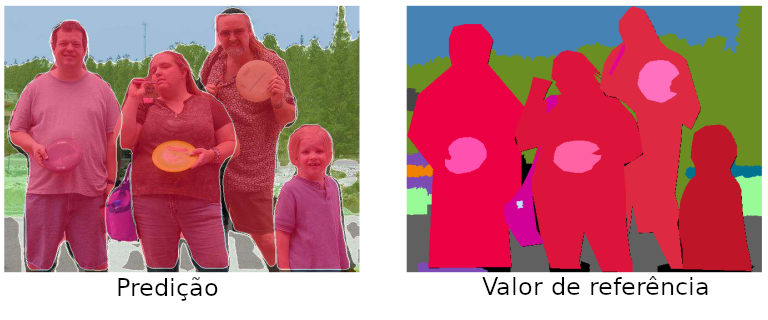
\includegraphics[width=1\linewidth]{recursos/imagens/panoptic/mau_adaptadas.png}
        \caption{Segmentação desalinhada.}
        \label{panoptic:fig:4.1}
    \end{subfigure}%
    ~ 

    \begin{subfigure}[t]{0.7\textwidth}
        \centering
        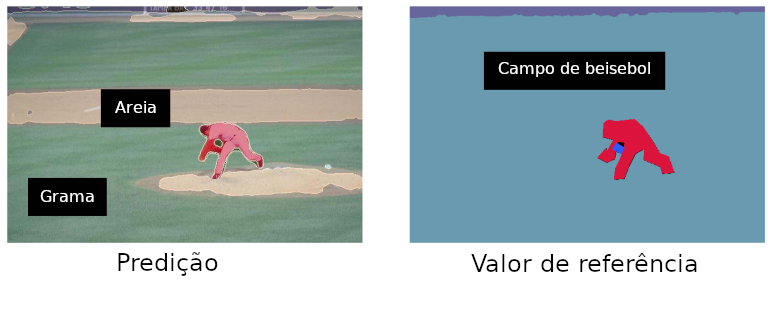
\includegraphics[width=1\linewidth]{recursos/imagens/panoptic/perda_contexto.png}
        \caption{Perda de contexto.}
        \label{panoptic:fig:4.2}
    \end{subfigure}%
    ~ 
    
    \begin{subfigure}[t]{0.7\textwidth}
        \centering
        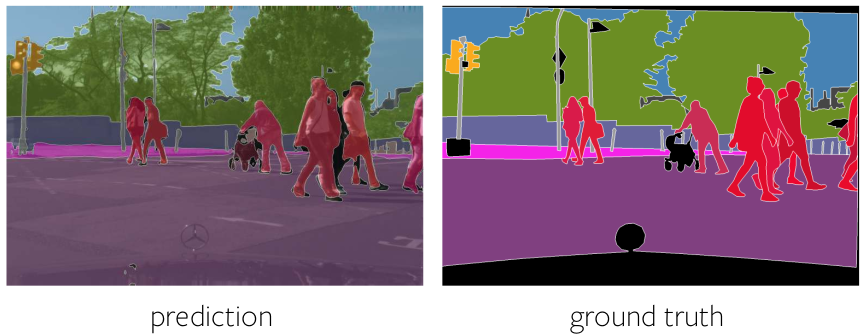
\includegraphics[width=1\linewidth]{recursos/imagens/panoptic/mau_alinhamento.png}
        \caption{Mau alinhamento.}
        \label{panoptic:fig:4.3}
    \end{subfigure}

    \vspace*{1 cm}
    Fonte: retirado e adaptado de \cite{Christoph2019}.
\end{figure}

Dessa forma, nas Tabelas \ref{conclusion:table:1} e \ref{conclusion:table:2}, é possível observar e comparar os métodos disponíveis para o trabalho com segmentações panópticas, destacando que os métodos foram realizadas nos conjuntos de dados COCO \cite{Lin2014} e Cityscape \cite{Cordts2016}, sendo estas os principais conjuntos de dados, como relatado na Seção \ref{panoptic:dataset}. Adicionalmente, foi gerada uma terceira tabela (Tabela \ref{conclusion:table:3}), que conta com trabalhos realizados no conjunto Mapillary Vistas \cite{Neuhold2017_ICCV}, a fim de que seja possível demonstrar a maior quantidade de trabalhos, redes neurais e métodos já disponíveis.

Ainda, quanto as Tabelas \ref{conclusion:table:1}, \ref{conclusion:table:2} e \ref{conclusion:table:3}, vale citar que as mesmas são compostas pelos métodos desenvolvidos e sua referência, as redes bases, as métricas de qualidade $PQ$ e $PC$, expressas nas equações \ref{panoptic:eq:1} e \ref{panoptic:eq:3}, respectivamente, $RQ$ e $SQ$, assim como a aplicação da métrica de $PQ$ para \textit{things} e \textit{stuffs}.

\begin{table}[H]
    \centering
    \caption{Comparação de desempenho no \textit{dataset} COCO  para segmentação panótica.}
    \label{conclusion:table:1}
    \resizebox{\textwidth}{!}{
    \begin{tabular}{l|l|l|l|l|l|l|l}
    \textbf{Métodos}                  &  \textbf{Rede Base}                 &  \textbf{PQ} &  \textbf{PQ-\textit{Thing}}    &    \textbf{PQ-\textit{Stuff}} &  \textbf{SQ} &  \textbf{RQ} &  \textbf{PC}  \\ \hline
    SOGNet\cite{Yang2020}             &  ResNet-50  \cite{He2016}           &   $43,7$     &  $50,6$                        &    $33,2$                     &  $78,7$      &   $53,5$     &   -       \\
    UPSNet\cite{Xiong2019}            &  ResNet-50  \cite{He2016}           &   $42,5$     &  $48,6$                        &    $33,4$                     &  -           &   -          &   -       \\
    OANet\cite{Liu2019}               &  ResNet-101 \cite{He2016}           &   $41,3$     &  $50,4$                        &    $27,7$                     &  -           &   -          &   -       \\
    OCFusion\cite{Lazarow2020}        &  ResNet-50  \cite{He2016}           &   $41,0$     &  $49,0$                        &    $29,0$                     &  $77,1$      &   $50,6$     &   -       \\
    Panoptic FPN\cite{Kirillov2019}   &  ResNet-101 \cite{He2016}           &   $40,9$     &  $48,3$                        &    $29,7$                     &  -           &   -          &   -       \\
    AUNet\cite{Li2019}                &  ResNet-50  \cite{He2016}           &   $39,6$     &  $49,1$                        &    $25,2$                     &  -           &   -          &   -       \\
    AdaptIS\cite{Sofiiuk2019}         &  ResNet-101 \cite{He2016}           &   $37,0$     &  $41,8$                        &    $29,9$                     &  -           &   -          &   -       \\
    DeeperLab\cite{Yang2019}          &  Xception-71 \cite{Chollet2017}     &   $34,3$     &  $37,5$                        &    $29,6$                     &  $77,1$      &   $43,1$     &   $56,8$ 
    \end{tabular}}

    \vspace*{1 cm}
    Fonte: retirado e adaptado de \cite{Li2020Awesome-Panoptic-Segmentation}.
\end{table}

\begin{table}[H]
    \centering
    \caption{Comparação de desemprenho no \textit{dataset} Cityscape para segmentação panótica.}
    \label{conclusion:table:2}
    \resizebox{\textwidth}{!}{
    \begin{tabular}{l|l|l|l|l|l|l|l}
    \textbf{Métodos}                   &    \textbf{Rede Base}            &  \textbf{PQ}     &  \textbf{PQ-\textit{Thing}}  &  \textbf{PQ-\textit{Stuff}}  & \textbf{SQ}  &  \textbf{RQ} &  \textbf{PC} \\ \hline
    Panoptic\cite{Kirillov2019a}       &  -                               &  $61,2$          &  $66,4$                      &  $54,0$                      &  $80,9$      &  $74,4$      &  -           \\
    AdaptIS\cite{Sofiiuk2019}          &  ResNet-101 \cite{He2016}        &  $60,6$          &  $58,7$                      &  $64,4$                      &  -           &  -           &  -           \\
    SOGNet\cite{Yang2020}              &  ResNet-50  \cite{He2016}        &  $60,0$          &  $56,7$                      &  $62,5$                      &  -           &  -           &  -           \\
    Seamless\cite{Porzi2019}           &  ResNet-50  \cite{He2016}        &  $59,8$          &  $53,4$                      &  $64,5$                      &  -           &  -           &  -           \\
    UPSNet\cite{Xiong2019}             &  ResNet-50  \cite{He2016}        &  $59,3$          &  $54,6$                      &  $62,7$                      &  $79,7$      &  $73,0$      &  -           \\
    TASCNet\cite{Lazarow2020}          &  ResNet-101 \cite{He2016}        &  $59,2$          &  $56  $                      &  $61,5$                      &  -           &  -           &  -           \\
    AUNet\cite{Li2019}                 &  ResNet-101 \cite{He2016}        &  $59,0$          &  $54,8$                      &  $62,1$                      &  -           &  -           &  -           \\
    Panoptic FPN\cite{Kirillov2019}    &  ResNet-101 \cite{He2016}        &  $58,1$          &  $52,0$                      &  $62,5$                      &  -           &  -           &  -           \\
    DeeperLab\cite{Yang2019}           &  Xception-71\cite{Chollet2017}   &  $56,5$          &  -                           &  -                           &  -           &  -           &  $75,6$      
    \end{tabular}}

    \vspace*{1 cm}
    Fonte: retirado e adaptado de \cite{Li2020Awesome-Panoptic-Segmentation}.
\end{table}

\begin{table}[H]
    \centering
    \caption{Comparação de desempenho no \textit{dataset} Mapillary.}
    \label{conclusion:table:3}
    \resizebox{\textwidth}{!}{
    \begin{tabular}{l|l|l|l|l|l|l|l}
    \textbf{Métodos}                      & \textbf{Rede Base}                & \textbf{PQ}  & \textbf{PQ-\textit{Thing}} & \textbf{PQ-\textit{Stuff}} &    \textbf{SQ}    &    \textbf{RQ} &    \textbf{PC} \\ \hline
    Panoptic\cite{Kirillov2019a}          & -                                 & $38,3$       & $41,8$                     & $35,7$                     & $73,6$            & $47,7$         & -              \\
    Seamless\cite{Porzi2019}              & ResNet-50  \cite{He2016}          & $37,2$       & $33,2$                     & $42,5$                     & -                 & -              & -              \\
    AdaptIS\cite{Sofiiuk2019}             & ResNet-101 \cite{He2016}          & $33,4$       & $28,3$                     & $40,3$                     & -                 & -              & -              \\
    TASCNet\cite{Lazarow2020}      & ResNet-101 \cite{He2016}          & $32,6$       & $31,3$                     & $34,4$                     & -                 & -              & -              \\
    DeeperLab\cite{Yang2019}              & Xception-71 \cite{Chollet2017}    & $32,0$       & -                          & -                          & -                 & -              & $55.3$    
    \end{tabular}}

    \vspace*{1 cm}
    Fonte: retirado e adaptado de \cite{Li2020Awesome-Panoptic-Segmentation}.
\end{table}

A partir das Tabelas 3 a 5, é possível observar que a maioria dos métodos desenvolvidos trabalha com a ResNet-50 ou ResNet-101 \cite{He2016}, com exceção do método DeeperLab \cite{Yang2019}, que também se destaca por ser a única que trabalha com a métrica $PC$ (Equação \ref{panoptic:eq:3}).

Outrossim, vale observar que o valor de $PQ$ (Equação \ref{panoptic:eq:1}) em qualquer uma das três tabelas não é superior a $61,2$, independente do método adotado, bem como é visível que o valor de $PQ-\textit{Thing}$ não é superior a  $66,4$ independente do conjunto ou método, mas é superior à métrica de $PQ-\textit{Stuff}$, o que possui relação com as anotações inconsistentes realizadas nos conjuntos de dados, como é exposto por \cite{Kirillov2019a}.

Por fim, propostas que complementem as dificuldades citadas na Seção \ref{panoptic:conclusion} podem ser exploradas com o uso de técnicas de \textit{deep learning}, técnicas artesanais de processamento digitais de imagem (como os citados por \cite{pedrini2008analise}), tal como a unificação de modelos e arquiteturas (como proposto por \cite{Liu2019}) citadas nesse trabalho, de modo que às métricas de $PQ$ e $PC$ sejam aumentadas entre os conjuntos de dados.